%\documentclass[preprint,prl,superscriptaddress]{revtex4-1}
%\documentclass[twocolumn,nofootinbib]{nature}
\documentclass[onecolumn,pra,superscriptaddress,nofootinbib]{revtex4-1}

% packages
\usepackage[dvips]{graphicx} % for figures
\usepackage{amsfonts,amssymb,amscd,amsmath,amsthm}
\usepackage{enumerate}
\usepackage{epsfig}
\usepackage{subfigure}
\usepackage{xcolor}
%\usepackage[expert]{mathdesign}

\newcommand{\bra}[1]{\mbox{$\left\langle #1 \right|$}}
\newcommand{\ket}[1]{\mbox{$\left| #1 \right\rangle$}}
\newcommand{\braket}[2]{\mbox{$\left\langle #1 | #2 \right\rangle$}}
\newcommand{\ketbra}[2]{\mbox{$\left\vert #1\right\rangle \left\langle #2\right\vert$ }}
\newcommand{\Tr}{\mathrm{Tr}}
\newcommand{\bfone}{\mathbf{I}}


\newtheorem{theorem}{Theorem}
\newtheorem{lemma}{Lemma}
\newtheorem{corollary}{Corollary}
\newtheorem{claim}{Claim}
\newtheorem{conjecture}{Conjecture}
\newtheorem*{observation}{Observation}
\newtheorem{definition}{Definition}

\begin{document}

\title{Lecture 2: two-qubit system}

%% For REVTeX it is possible to automate superscript and e-mail callouts with the superscriptaddress option; see REVTeX4 documentation.


\author{Xiongfeng Ma}
\email{xma@tsinghua.edu.cn}
\affiliation{Center for Quantum Information, Institute for Interdisciplinary Information Sciences, Tsinghua University, Beijing 100084, China}


\begin{abstract}
In the last chapter, we have learned about one qubit system. Here, we shall learn about a two-qubit system. It turns out two-qubit system has much more fun. It will take three weeks for us to cover these materials. Guess how many qubits we can cover by the end of the course?

Two-qubit state, mixed state, Bloch ``ball", positive-operator valued measure (POVM); Super operator, purification of mixed state and POVM; Using teleportation for operation (Gottesman-Chuang'99), remote state preparation; Bell's inequality, CHSH/CH/Eberhard inequality; experiment development and loopholes, entanglement; Quantum dense coding, teleportation (experiment development);
\end{abstract}

%\ocis{(270.5565) Quantum communications; (270.5568) Quantum cryptography.}


\maketitle %% required

\section{Review: one-qubit System}
\begin{enumerate}
\item{state: ray.}
\item{normalize state: vector.}
\item{representation way: $\ket{u}=\cos{\frac{\theta}{2}}+e^{i\varphi}\sin{\frac{\theta}{2}}$. (Bloch Sphere\footnote{No standard way to visualize two or more qubits system until now.})}
\item{density matrix: $\rho = \sum_i\lambda_i\ket{\phi_i}\bra{\phi_i}$.\footnote{why we can't distinguish $\ket{u}$ and $e^{i\theta}\ket{u}$? because $\ket{u}\bra{u}=e^{i\theta}\ket{u}\bra{u}e^{-i\theta}$. Their density matrices are always the same.}}
\item{$\rho^{+} = \rho, Tr(\rho) = 1.$}
\item{$\forall \ket{\phi}, \bra{\phi}\rho\ket{\phi} \geq 0$.\footnote{By physical meaning of the measurement}}
\item{For pure qubit, Assume $\rho = \ket{\phi}\bra{\phi}$, we have $\rho^2 = \rho.$ Also, we can get the eigenvalues and eigenvectors of $\rho$ (Assume $\ket{\Phi}$ is orthogonal of $\ket{\phi}$):
\begin{equation}
\begin{aligned}
\rho\ket{\phi} = \ket{\phi}\braket{\phi}{\phi} = \ket{\phi}.\\
\rho\ket{\Phi} = \ket{\phi}\braket{\phi}{\Phi} = 0.
\end{aligned}
\end{equation}}

\item{$\bra{\psi}M\ket{\psi} = Tr(\bra{\psi}M\ket{\psi}) = Tr(M\ket{\psi}\bra{\psi}) = Tr(M\rho).$\footnote{$Tr(AB)=\sum_{i}\sum_j a_{ij}b_{ji} = \sum_{i}\sum_j b_{ij}a_{ji} = Tr(BA)$.}}
\end{enumerate}
\subsection{Bloch sphere}
A useful representation of the state of a single qubit is the Bloch sphere representation. Since the overall phase is irrelevant, a pure state of a qubit can be written as
\begin{equation} \label{eq:BlochSphere}
\begin{aligned}
\ket{u} = \cos\frac{\theta}{2}\ket{0}+e^{i\varphi}\sin\frac{\theta}{2}\ket{1}.
\end{aligned}
\end{equation}
Therefore, it is convenient to represent it as a vector living the surface of a unit sphere with the spherical coordinate $(r=1,\theta,\varphi)$.

\begin{figure}[tbh]
\centering \resizebox{4cm}{!}{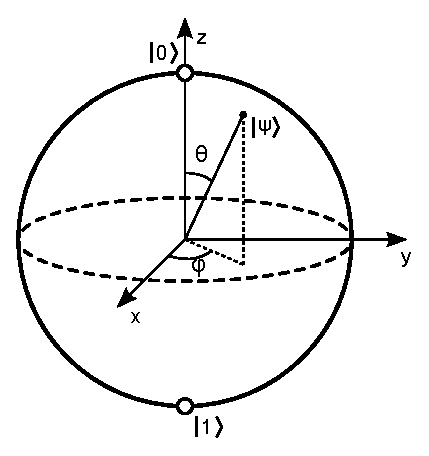
\includegraphics{epsBlochSphere.eps}}
\caption{Bloch sphere.} \label{fig:BlochSphere}
\end{figure}

In general, a qubit might be in a mixed state, and then it will be within the Bloch sphere instead on the surface. In general, the density matrix of a qubit can be written as
\begin{equation} \label{eq:rhoBloch}
\begin{aligned}
\rho &= \frac12(\sigma_0+\vec{P}\cdot \vec{\sigma}) \\
&= \frac12
    \begin{pmatrix}
      1+P_z&P_x-iP_y\\
      P_x+iP_y&1-P_z
    \end{pmatrix}
\end{aligned}
\end{equation}
where $\vec{P}=(P_x,P_y,P_z)$ is a vector and $|\vec{P}|\le1$. When $|\vec{P}|=1$, Eq.~\eqref{eq:rhoBloch} represents a pure qubit.


\section{Notations}
Matrix tensor product $\otimes$,
%consider two matrices,
%\begin{equation} \label{2qubit:2mat}
%\begin{aligned}
%\[
%\begin{pmatrix}
%    a_{1,1} & a_{1,2} \\
%    a_{2,1} & a_{2,2}
%\end{pmatrix}
%
%\begin{pmatrix}
%    b_{1,1} & b_{1,2} \\
%    b_{2,1} & b_{2,2}
%\end{pmatrix}.
%\]
%\end{aligned}
%\end{equation}
the tensor product of two matrices is
\begin{equation} \label{2qubit:tensorproduct}
\begin{aligned}
  \begin{bmatrix}
    a_{1,1} & a_{1,2} \\
    a_{2,1} & a_{2,2} \\
  \end{bmatrix}
\otimes
  \begin{bmatrix}
    b_{1,1} & b_{1,2} \\
    b_{2,1} & b_{2,2} \\
  \end{bmatrix}
=
  \begin{bmatrix}
    a_{1,1}  \begin{bmatrix}
              b_{1,1} & b_{1,2} \\
              b_{2,1} & b_{2,2} \\
            \end{bmatrix} & a_{1,2}  \begin{bmatrix}
                                      b_{1,1} & b_{1,2} \\
                                      b_{2,1} & b_{2,2} \\
                                    \end{bmatrix} \\
     & \\
    a_{2,1}  \begin{bmatrix}
              b_{1,1} & b_{1,2} \\
              b_{2,1} & b_{2,2} \\
            \end{bmatrix} & a_{2,2}  \begin{bmatrix}
                                      b_{1,1} & b_{1,2} \\
                                      b_{2,1} & b_{2,2} \\
                                    \end{bmatrix} \\
  \end{bmatrix}
=
  \begin{bmatrix}
    a_{1,1} b_{1,1} & a_{1,1} b_{1,2} & a_{1,2} b_{1,1} & a_{1,2} b_{1,2} \\
    a_{1,1} b_{2,1} & a_{1,1} b_{2,2} & a_{1,2} b_{2,1} & a_{1,2} b_{2,2} \\
    a_{2,1} b_{1,1} & a_{2,1} b_{1,2} & a_{2,2} b_{1,1} & a_{2,2} b_{1,2} \\
    a_{2,1} b_{2,1} & a_{2,1} b_{2,2} & a_{2,2} b_{2,1} & a_{2,2} b_{2,2} \\
  \end{bmatrix}.
\end{aligned}
\end{equation}


Here, we simplify denote it as
\begin{equation} \label{2qubit:tensorsimp}
\begin{aligned}
\ket{\phi}\otimes\ket{\psi} = \ket{\phi}\ket{\psi}\\
\end{aligned}
\end{equation}


\subsection{Trace}
Trace $Tr(\rho)$: summation of the diagonal terms.

Partial trace $Tr_B(\rho_{AB})$: Assume A is n-dimension state, B is m-dimension state, then $\rho_{AB}$ can be regarded as a $nm \times nm$ matrix. $Tr_B(\rho_{AB})$ is a $n\times n$ matrix, where
\begin{equation} \label{2qubit:partialtr}
\begin{aligned}
(Tr_B(\rho_{AB}))_{ij} = \sum_{k=1}^{m}(\rho_{AB})_{ik, jk} \\
\end{aligned}
\end{equation}
Particularly, $Tr_B(A \otimes B) = Tr(B)A.$


\section{Two-qubit system}

\subsection{an interesting ``paradox"}
When considering a two qubits state which is written as
\begin{equation} \label{2qubit:4Bell0011}
\begin{aligned}
\ket{\psi}_{AB}=\frac{1}{\sqrt2}(\ket{0}_{A}\ket{0}_{B}+\ket{1}_{A}\ket{1}_{B}).\\
\end{aligned}
\end{equation}
When measure the system $A$ in the $Z$ basis, with probability $1/2$, the measurement result is $\ket{0}$ and the prepared state is $\ket{0}_A\ket{0}_B$. With probability $1/2$, the measurement result is $\ket{1}$ and the prepared state is $\ket{1}_A\ket{1}_B$. Naively, one might express system $A$ in the state of
\begin{equation} \label{2qubit:plus}
\begin{aligned}
\ket{\psi}_A = \frac{1}{\sqrt{2}}(\ket{0} + \ket{1}) = \ket{+}.
\end{aligned}
\end{equation}


Consider another two-qubit state,
\begin{equation} \label{2qubit:4Bellppmm}
\begin{aligned}
\ket{\psi}_{AB}=\frac{1}{\sqrt2}(\ket{+}_{A}\ket{+}_{B}+\ket{-}_{A}\ket{-}_{B}).\\
\end{aligned}
\end{equation}
Following the same naive argument, we should have
\begin{equation} \label{2qubit:0}
\begin{aligned}
\ket{\psi}_A = \frac{1}{\sqrt{2}}(\ket{+} + \ket{-}) = \ket{0}.
\end{aligned}
\end{equation}

But, on the other hand,
\begin{equation} \label{2qubit:Belleq}
\begin{aligned}
\ket{\psi}_{AB}&=\frac{1}{\sqrt2}(\ket{0}_{A}\ket{0}_{B}+\ket{1}_{A}\ket{1}_{B}) \\
 &= \frac{1}{2\sqrt2}(\ket{+}+\ket{-})(\ket{+}+\ket{-})+\frac{1}{2\sqrt2}(\ket{+}-\ket{-})(\ket{+}-\ket{-})\\
 &= \frac{1}{\sqrt2}(\ket{+}_A\ket{+}_B+\ket{-}_A\ket{-}_B).
\end{aligned}
\end{equation}
So now we have: $\ket{0} = \ket{+}$. What is wrong?


\textbf{Explanation:} The key of the above paradox is that $\ket{\psi}_A$ is not a pure state any more, we only can write it as a density matrix. The density operator of subsystem A is given by
\begin{equation} \label{4BellZ}
\begin{aligned}
\rho_A=tr_B(\ket{\psi}_{AB}\bra{\psi}_{AB})=\frac{1}{\sqrt{2}}(\ket{0}\bra{0}+\ket{1}\bra{1}).\\
\end{aligned}
\end{equation}


\subsection{EPR paradox}
Alice and Bob share a two qubits system:
$$
\ket{\psi}_{AB} = \frac{1}{\sqrt2}(\ket{0}_{A}\ket{0}_{B}+\ket{1}_{A}\ket{1}_{B}).
$$
Alice gets qubit A, Bob gets qubit B. Then Alice goes to a planet which far from Bob. Then if Alice wants to tell 0 to B, she measures A in $\ket{+/-}$ basis; if she wants to tell 1 to B, she measures A with $\ket{0/1}$ basis.

We assume that after measurement for A, Alice gets $\ket{0}$. Then
for Bob, he measures B after a while with basis $\ket{0/1}$, if he gets $\ket{0}$ with probability 1, he can say Alice wants to tell him 0.

So by this process, we transform information which is faster than light. What's the problem?

\textbf{Explanation:} For Bob, if he gets $\ket{0}$, he doesn't know which basis Alice uses. Because if Alice chooses $\ket{0/1}$ basis, Bob has $0.5$ probability to get $\ket{0}$; if Alice chooses $\ket{+/-}$ basis, Bob also has $0.5$ probability to get $\ket{0}$.

This experiments tells us, quantum has the \textbf{non-locality} and also \textbf{no-signalling} properties.
$$
\textit{Something are changed, but we do not know. We simply use the same state to describe the system.}
$$


\subsection{Density matrix of subsystem}

%%%%%%%%%%
%% From week2-2
For a bipartite system $\rho_{AB}$, the density matrix of subsystem A can be denoted as $Tr_B
(\rho_{AB})$. For example, $\vert\psi\rangle_{AB} = a\vert 0\rangle_A \vert 0\rangle_B + b \vert 1\rangle_A \vert 1\rangle_B$. Then $\rho_A = \Tr_B(\vert\psi\rangle_{AB}\langle\psi\vert_{AB}) = aa^* \vert 0\rangle \langle 0\vert + bb^*\vert 1\rangle \langle 1\vert$. In general, there are some properties of $\rho_A$:
\begin{itemize}
\item $\rho_A^\dagger = \rho_A$.
\item $\rho_A \geq 0$.
\item $\Tr(\rho_A) = 1$.
\end{itemize}

Comment: If $\rho_A$ is pure state, then $\rho_A^2 = \rho_A$, the purity $\Tr(\rho_A^2)\leq 1 \Rightarrow \Tr(\rho_A^2) =1 $.
\subparagraph{An example}
$\vert\psi\rangle_{AB} =  \vert 0\rangle_A \vert 0\rangle_B+\vert 1\rangle_A\vert 1\rangle_B = \vert+\rangle_A\vert +\rangle_B+\vert - \rangle_A\vert -\rangle_B$ has two representations. There are two cases to measure $\rho_A = \frac12 \bfone$.
\subparagraph{Case 1:} How to get $\rho_A = \frac12 ( \vert 0\rangle \langle 0\vert+\vert 1\rangle\langle 1\vert)$ ?
\begin{enumerate}

\item Prepare $\vert0\rangle\vert 0\rangle+\vert 1\rangle\vert 1\rangle$
\item Measure $B$ in $z=0$ and $z=1$
\item Given $z$-measure result. $A=\vert 0\rangle$ or $\vert 1\rangle$.
\item $\rho_{A1} = \frac12 \vert 0\rangle\langle 0\vert +\frac12 \vert 1\rangle\langle 1\vert$.
\end{enumerate}
\subparagraph{Case 2:} How to get $\rho_A = \frac12 (\vert+\rangle\langle +\vert+\vert - \rangle\langle -\vert)$?
\begin{enumerate}
\item Prepare $\vert+\rangle\vert +\rangle+\vert - \rangle\vert -\rangle$
\item measure $B$ in $x = \vert +\rangle$ and $x= \vert -\rangle$.
\item Given $x$-measure results, $A = \vert +\rangle$ or $\vert -\rangle$
\item $\rho_{A2} = \frac12 \vert +\rangle\langle +\vert +\frac12 \vert -\rangle\langle -\vert$.
\end{enumerate}

\subparagraph{}
$\rho_{A1} = \rho_{A2}$. From Alice's point of view, they are the same, although  Bob knows which of the two pure states it is. When Bob tells Alice the information of the state, the states collapses. (Information is physical; physics is informational.)

\subparagraph{Coherence (classical mixture or superposition).}
 $\vert\psi\rangle = \frac{1}{\sqrt2}(\vert 0\rangle+\vert 1\rangle), \vert \psi\rangle \langle \psi\vert = \frac12 \left[\begin{array}{cc}1 & 1\\1& 1\end{array}\right]$. If we measure in $x$ we always get the same.
But it is different for $\frac12 \vert 0\rangle\langle 0\vert +\frac12 \vert 1\rangle\langle 1\vert$ (which can be distinguished by measuring in $z$).

We prefer the pure state $\frac{1}{\sqrt2}(\vert 0\rangle+\vert 1\rangle)$ to generated randomness, because additional information can not change the state, while the other one can be attacked by measuring the entangled qubit.

Comment:  Given a pure state, we know every information in the system and can not change it by getting more information, since the entropy is already zero (not the case for general density matrix).
\subsection{The properties for general density matrix}
In general, the state is represented by a density operator.
In the case where the state of the subsystem is a ray, and we say that the state is
pure. Otherwise the state is mixed. If $\rho_A=\rho_A^2$, then $\ket{\psi_A}$ is a pure state. Otherwise, the density matrix of A is
$\rho_A=\sum_a p_a\ket{a}\bra{a}$, where $\sum_ap_a=1$, $0<p_a<1$. The trace distance $tr \rho_A^2=\sum_a p_a^2<\sum_ap_a=1$.

Properties of a general density matrix
\begin{enumerate}
\item
self-adjoint: $\rho_A=\rho_A^\dag$
\item
positivity: $\forall\ket{\psi}$, $\bra{\psi}\rho_A\ket{\psi}\ge0$
\item
completeness: $Tr(\rho_A)=1$
\end{enumerate}



\subsection{Schmidt decomposition}
For any pure state $\ket{\psi}_{AB}$ of a bipartite system, there are orthonormal bases $\{\ket{i}_A\}$ and $\{\ket{i�V�d}_B\}$ such that:
\begin{equation} \label{Schmidt decomposition}
\begin{aligned}
\ket{\psi}_{AB}=\sum_i\sqrt{p_i}\ket{i}_A\otimes\ket{i'}_B.
\end{aligned}
\end{equation}
The subsystems $A$ and $B$ have the same eigenvalues, $p_i$s. The number of $p_i$s is called the Schmidt number of $\ket{\psi}_{AB}$. We denote that the pure state is a entangled state when the the Schmidt number is greater than one. It is easy to see that the Bell states are entangled states.


%% week3
For pure $\ket{\psi}_{AB}x$, you can always find $\rho_A = \rho_B$ in any basis of $\rho_A$.

\subsection{Bell basis}
The dimension of the 2-qubit Hilbert space is 4. Thus, there are 4 basis states. Bell state basis is widely used, especially for the case involving entanglement. The 4 Bell states in the $Z$ basis are,
\begin{equation} \label{4BellZ}
\begin{aligned}
\Phi^+ &= \ket{00}+\ket{11} \\
\Phi^- &= \ket{00}-\ket{11} \\
\Psi^+ &= \ket{01}+\ket{10} \\
\Psi^- &= \ket{01}-\ket{10} \\
\end{aligned}
\end{equation}
in the $X$ basis are
\begin{equation} \label{4BellZ}
\begin{aligned}
\Phi^+ &= \ket{++}+\ket{--} \\
\Phi^- &= \ket{-+}+\ket{+-} \\
\Psi^+ &= \ket{++}-\ket{--} \\
\Psi^- &= \ket{-+}-\ket{+-} \\
\end{aligned}
\end{equation}
in the $Y$ basis are
\begin{equation} \label{4BellZ}
\begin{aligned}
\Phi^+ &= \ket{+i-i}+\ket{-i+i} \\
\Phi^- &= \ket{+i+i}+\ket{-i-i} \\
\Psi^+ &= -i(\ket{+i+i}-\ket{-i-i}) \\
\Psi^- &= i(\ket{+i-i}-\ket{-i+i}) \\
\end{aligned}
\end{equation}

Many interesting simple quantum information phenomenons come with Bell states, such as Bell's inequality, Teleportation, super dense coding, quantum key distribution, and Deutsch's algorithm.


\subsection{Qubit tomography}
Quantum state tomography is the process of reconstructing the quantum state for a quantum system by proper measurements. The quantum state can be pure (vector) or in general mixed (density matrix). A set of measurements is called tomographically complete if it can uniquely identify the state. That is, the measurement outcomes are able to provide all the information about the state. In the classical physics, it corresponds to system calibration.

Let us take qubit tomography for example. As given in Eq.~\eqref{eq:rhoBloch}, the $Z$ basis measure provides the information on $P_z$. By changing the $Z$ and $X$ basis, by the Hadamard transformation, we can conclude that the $X$ basis measure provides the information on $P_x$. Similarly, the $Y$ basis measure provides the information on $P_y$. Thus, $X$, $Y$, and $Z$ measurements is tomographically complete for a qubit. Another way to put this is,
\begin{equation} \label{eq:rho2tomo}
\begin{aligned}
\rho &= \frac12[tr(\rho)\sigma_0+tr(\sigma_x\rho)\sigma_x+tr(\sigma_y\rho)\sigma_y+tr(\sigma_z\rho)\sigma_z]. \\
\end{aligned}
\end{equation}
Now, let us move a bit further, tomography for $n$ qubits,
\begin{equation} \label{eq:rhontomo}
\begin{aligned}
\rho &= 2^{-n}\sum_{v_1,v_2,\dots,v_n\in\{0,x,y,z\}}tr(\sigma_{v1}\otimes\sigma_{v2}\otimes\cdots\otimes\sigma_{vn}\rho) \sigma_{v1}\otimes\sigma_{v2}\otimes\cdots\otimes\sigma_{vn},
\end{aligned}
\end{equation}
where the sum is over all possible the identity and Pauli matrices.

In another related concept, quantum process tomography, known quantum states are used to probe a quantum process to find out how the process can be described. Similarly, quantum measurement tomography works to find out what measurement is being performed.

The general principle behind quantum state tomography is that by repeatedly performing many different measurements on quantum systems described by identical density matrices, frequency counts can be used to infer probabilities, and these probabilities are combined with Born's rule to determine a density matrix which fits the best with the observations.

\section{Measurement}

\subsection{Projection-value measurement}
Projection-value measurement (PVM) are denoted by $\{M_m\}m$, such that
\begin{enumerate}
\item $\sum_m M_m^{\dag}M_m = I.$
\item $M_m = M_m^{\dag}.$
\item $M_mM_{m'} = \delta_{m,m'}M_m.$
\end{enumerate}

For example, $\{\ket{0}\bra{0}, \ket{1}\bra{1}\}$ is a projection-value measurement of one qubit system.

\subsection{Positive-operator value measurement}
Positive-operator value measurement (POVM) are denoted by $\{E_m\}_m$, satisfy
\begin{enumerate}
\item $\sum_m E_m = I.$
\item $E_m = E_m^{\dag}.$
\item $\forall \ket{\phi},~ \bra{\phi}E_m\ket{\phi}\geq 0.$
\end{enumerate}

For example, $\{\ket{0}\bra{0}\otimes I, \ket{1}\bra{1} \otimes I\}$ is a POVM of a two qubit system (actually it measures the first qubit in z basis).

PVM is the special case of POVM in the sense that $E_m = M_m^{\dag}M_m.$ We can understands the difference between the Positive Operator-Valued Measure (POVM) and PVM with the same sense that a density matrix is to a pure state. The POVM can be used to describe the effect of PVM acts on a large system.

In general, the probability to get $m$ in a measurement is
\begin{equation}
\Pr(m) = \Tr(E_m\rho).
\end{equation}

New density matrix $\rho'$ after the measurement is
\begin{equation}
\rho' = \frac{E_m \rho}{\Tr(E_m\rho)}.
\end{equation}

\subsection{one-qubit tomography}
How to decide $\rho = \frac12 (I+\vec{P}\cdot\vec{\sigma})$ by measurements?

We have $P_i = \Tr(\rho\sigma_i)(i = x,y,z)$, i.e.
\begin{gather*}
\rho = \frac12 \left( \Tr(\rho I)I + \sum_{i=x,y,z}\Tr(\sigma_i \rho)\sigma_i\right).
\end{gather*}

In order to get $P_x$ by measurements, we measure in $x$-basis: $\pm$. There is
\begin{equation}
\begin{aligned}
P_x &= \Tr(\sigma_x\rho)\\
	&= \Tr((\braket{+}{+}-\braket{-}{-})\rho)\\
	&= \Tr(\bra{+}\rho\ket{+}-\bra{-}\rho\ket{-})\\
	&= \Pr(+) - \Pr(-).
\end{aligned}
\end{equation}

In experiments, we count the number of $+$ and $-$, then calculate $\Pr(+)-\Pr(-)=P_x$.

By similar calculation, we have
\begin{equation}
\Pr(+i)-\Pr(-i) =  P_y, \Pr(0)-\Pr(1) = P_z.
\end{equation}

\subsection{multipul-qubits tomography}
We generalize the way of one qubi tomorgraphy: Use $\sigma_i\otimes\sigma_j$ to measure $\rho_{AB}$.
\begin{equation}
\rho_{AB} = \frac14\sum
_{i,j\in\{I,x,y,z\}}
P_{ij}\sigma_i\otimes\sigma_j.
\end{equation}

Similarly, we can calculate $P_{II}$ directly:
\begin{equation}
\begin{aligned}
\Tr(\rho_{AB}) &=\frac14\sum_{i,j}P_{ij}\Tr(\sigma_i\otimes\sigma_j) \\
&= \frac14\sum_{i,j}P_{ij}\Tr(\sigma_i)\Tr(\sigma_j) \\
&= \frac14P_{II}\Tr(\sigma_I)\Tr(\sigma_I) \\
&= P_{II}.\\
\end{aligned}
\end{equation}
Because $\Tr(\rho_{AB}) = 1$, there is
$P_{II} = 1$.

In general, there is $P_{ij} = \Tr(\sigma_{i}\otimes \sigma_j \rho)$:
\begin{equation}
\begin{aligned}
 \Tr(\rho \sigma_i\otimes\sigma_j) &= \frac14\Tr(\sum_{i'j'}P_{i'j'}(\sigma_{i'}\otimes\sigma_{j'})(\sigma_i\otimes\sigma_j)) \\
&= \frac14\sum_{i'j'}P_{i'j'}\Tr(\sigma_i'\sigma_i)
\Tr(\sigma_j'\sigma_j)\\
&= \frac14P_{ij}\Tr(\sigma_i\sigma_i)\Tr(\sigma_j\sigma_j)\\
&=\frac14P_{ij}\Tr(\sigma_I)\Tr(\sigma_I)\\
&=P_{ij}.
\end{aligned}
\end{equation}

\subparagraph{n-qubit system.}
$\bigotimes_{v_i=\in\{I,x,y,z\}} \sigma_{v_i}, \rho = \sigma_{v_i}\Tr(\rho\bigotimes_{v_i}\sigma_{v_i})\bigotimes(\sigma_{v_i}).$
$3^n$ measurement should be performed, but the DOF is less, so this tomography is not optimal.

\subparagraph{Individual measurement:} $4^n$ terms (nothing for $I$).

\subsection{Joint measurement (BSM: Bell-state measurement)}
Bell state measurement is the measurement which use the Bell states as basis: $\phi^{\pm} = \ket{00}\pm\ket{11}, \psi^{\pm} = \ket{01}\pm\ket{10}$.

We can use Hadamard operation and C-NOT operation to realize BSM.

The Hadamard operation is
\begin{equation}
H = \frac{1}{\sqrt{2}}\begin{pmatrix} 1 & 1\\ 1 &-1
\end{pmatrix}
\end{equation}
where $H\ket{+} = \ket{0}, H\ket{-} = \ket{1}.$

The C-NOT operation is $4 \times 4$ unitary matrix:
\begin{gather}
\text{C-NOT} = \frac12\left(\begin{array}{cccc}
1&0&0&0\\
0&1&0&0\\
0&0&0&1\\
0&0&1&0
\end{array}\right).
\end{gather}
where
\begin{eqnarray}
\text{C-NOT}\ket{0}\ket{0} &= \ket{0}\ket{0}\\
\text{C-NOT}\ket{0}\ket{1} &= \ket{0}\ket{1}\\
\text{C-NOT}\ket{1}\ket{0} &= \ket{1}\ket{1}\\
\text{C-NOT}\ket{1}\ket{1} &= \ket{1}\ket{0}\\
\end{eqnarray}

We define unitary matrix
\begin{equation}
U = (H \otimes I)\text{C-NOT}.
\end{equation}

Then, there is
\begin{eqnarray}
U(\ket{00}+\ket{11}) &= (H \otimes I)\ket{+0} &= \ket{00}\\
U(\ket{00}-\ket{11}) &= (H \otimes I)\ket{-0} &= \ket{10}\\
U(\ket{01}+\ket{10}) &= (H \otimes I)\ket{+1} &= \ket{01}\\
U(\ket{01}-\ket{10}) &= (H \otimes I)\ket{-1} &= \ket{11}\\
\end{eqnarray}
Then measure in $z$-basis.

\section{quantum channel}
The quantum channel is also called ``super operator". The super means that the map takes operators to operators, rather than vectors to vectors. Unitary evolution on $\mathcal{H}_A\otimes\mathcal{H}_B $ will not in general appear to be unitary if we restrict our attention to $\mathcal{H}_A$ alone. Rather, evolution in HA will be described by a quantum channel, (which can be inverted by another channel only if unitary). A general channel $\mathcal{E}$ has an operator-sum representation:
\begin{equation} \label{eq:channel}
\begin{aligned}
\mathcal{E}(\rho)=\sum_aM_a\rho M_a^\dag,\\
\sum_aM_a^\dag M_a=I.\\
\end{aligned}
\end{equation}


\section{Ensembles and purification}
A mixed state of a system A can be prepared as an ensemble of pure states in
many different ways, all of which are experimentally indistinguishable if
we observe system A alone.

For any density matrix $\rho_A$, we can find its Schmidt-decomposition:
\begin{equation} \label{eq:Ensembles}
\begin{aligned}
\rho_A &=\sum_ip_i\ket{\psi_i}\bra{\psi_i}, \\
\end{aligned}
\end{equation}
with $\sum p_i=1$.

For any such $\rho_A$,  we can construct a ``purification" of $\rho_A$, $\ket{\Psi_1}_{AB}$,
\begin{equation} \label{eq:purification}
\begin{aligned}
\ket{\Psi_1}_{AB}=\sum_i \sqrt{p_i}\ket{\psi_i}_A\ket{\alpha_i}_B,
\end{aligned}
\end{equation}
where $\{\ket{\alpha_i}_B\}$ are mutually orthogonal and normalized.

The relation between two purifications, $\ket{\Psi_1}_{AB}$ and $\ket{\Psi_2}_{AB}$, is given by,
\begin{equation} \label{eq:purifications}
\begin{aligned}
\ket{\Psi_1}_{AB}=(I_A\otimes U_B)\ket{\Psi_2}_{AB},
\end{aligned}
\end{equation}
the two states differ by an unitary change of basis acting in $\mathcal{H}_B$ alone (homework).

For example, purify the density matrix:
$$
\rho = \left(\begin{array}{cc}
\frac49 &\frac{1}{100}\\
\frac{1}{100}&\frac59\\
\end{array}\right)$$.

First step, find Schmidt-decomposition of $\rho$:
$$
\rho = \lambda_0 \ket{i_0}\bra{i_0} + \lambda_1 \ket{i_1}\bra{i_1}.
$$
where $\lambda_0, \lambda_1$ are eigenvalues of $\rho$, and $i_0, i_1$ are the corresponding eigenvectors.

Second step, the purification of $\rho$ is
$$
\ket{\psi_{AB}} = \sqrt{\lambda_0}\ket{i_0}\ket{i_0
'}+\sqrt{\lambda_1}\ket{i_1}\ket{i_1
'}.
$$
\section{Bell's inequalities}
Bell's theorem \cite{bell1964einstein}: no physical theory of local hidden variables can ever reproduce all of the predictions of quantum mechanics.

\subsection{Clauser-Horne-Shimony-Holt inequality}
One of the most well known Bell's inequality is the Clauser-Horne-Shimony-Holt (CHSH) inequality \cite{Clauser1969CHSH}. There are many ways to express it. We study it from a quantum game point of view.

As shown in Fig.~\ref{Fig:BellTest}, two space-like separated parties, Alice and Bob, randomly choose input bit settings $x$ and $y$ and generate outputs bits $a$ and $b$ based on their inputs and pre-shared quantum ($\rho$) and classical ($\lambda$) resources, respectively. The probability distribution $p(a,b|x,y)$,  obtaining outputs $a$ and $b$ conditioned on inputs $x$ and $y$, are determined by specific strategies of Alice and Bob. By assuming that the input settings $x$ and $y$ are chosen fully randomly and equally likely, the CHSH inequality is defined by a linear combination of the probability distribution $p(a,b|x,y)$ according to
\begin{equation}\label{eq:Bell}
  S = \sum_{a,b,x,y} (-1)^{a\oplus b + x\cdot y}p(a,b|x,y) \leq S_C = 2,
\end{equation}
where the plus operation $\oplus$ is modulo 2, $\cdot$ is numerical multiplication, and $S_C$ is the (classical) bound of Bell value $S$ for all LHVMs.

\begin{figure}[hbt]
\centering \resizebox{4cm}{!}{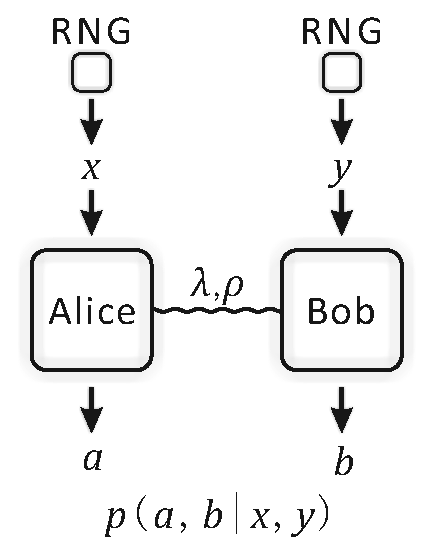
\includegraphics{epsBell1.eps}}
\caption{Bipartite Bell inequality. The inputs of Alice and Bob, $x$ and $y$,  are decided by perfect random number generators (RNGs), which produce uniformly distributed random numbers.} \label{Fig:BellTest}
\end{figure}

Similarly, there is an achievable bound $S_Q = 2\sqrt{2}$ for the quantum theory \cite{cirel1980quantum}. In this case, a violation of the classical bound $S_C$ indicates the need for alternative theories other than LHVMs, such as quantum theory. For general no signalling (NS) theories \cite{prbox}, denote the corresponded upper bound as $S_{NS} = 4$. It is straightforward to see that $S_{NS} \geq S_Q\geq S_C$.

Different strategies impose different constraints on the probability distribution.
\begin{itemize}
  \item Classical: $p(a,b|x,y) = \sum_\lambda q(\lambda)p(a|x,\lambda)p(b|y,\lambda)$
  \item Quantum: $p(a,b|x,y) = \mathrm{Tr}[\rho_{AB}M_a^x\otimes M_b^y]$
  \item No-signaling: $\sum_a p(a,b|x,y) = \sum_a p(a,b|x',y), \sum_b p(a,b|x,y) = \sum_b p(a,b|x, y')$
\end{itemize}
\subsection{Experiment loopholes}
Since the first experiment in the early 1980s \cite{Aspect1982PhysRevLett.49.91}, lots of lab demonstrations of the CHSH inequality have been presented. In practice, the conclusion of the violation of a Bell test is conditioned on several assumptions. %\subsection{Experiment problems}
Experimental demonstrations suffer from three major loopholes.

\emph{Locality loophole:}
The measurement events of Alice and Bob should be space-like separated. If this condition is not satisfied, Bell's inequality can be violated even with LHVMs by signaling. This loophole can be closed by separating Alice and Bob sufficient apart such that the measurement events are space-like separated. In experiment, this loophole is closed in optical systems \cite{Weihs98} and shown to be promising to be closed in atomic systems \cite{hofmann2012heralded}.

\emph{Efficiency loophole:}
The detection efficiency must be higher than a threshold to ensure the violation without assuming fair sampling. In the famous CH or Eberhard \cite{Eberhard93} test, it is shown that the efficiency should be at least 2/3 for each party, which is also proved to be a tight bound \cite{Massar03, Wilms08} for all bipartite Bell test with two inputs. The efficiency loophole can be closed in different realizations \cite{rowe2001experimental,Christensen13,giustina2013bell}.

\emph{Randomness loophole:}
The inputs $x$ and $y$ should be random and thus cannot be predetermined. Also, we require $x$ and $y$ to be uncorrelated to each other and also from different runs \cite{Koh12, Pope13}. In experiment, this loophole cannot be closed perfectly, as we can never unconditionally certify the randomness without a faithful Bell test, which in turn requires faithful randomness. Thus, we have to assume the existence of a true random seed. In practice, we can make use of independent random number generators, such as causally disconnected cosmic photons \cite{Gallicchio14}. On the other hand, if we can characterize the randomness well, we can also check whether the input randomness satisfy the requirement \cite{Hall10,Koh12,Pope13,Yuan15,Yuan15b} that guarantee the conclusion even with imperfect randomness input.


\subsection{CH and Eberhard's inequality}
In the bipartite scenario, a general Bell test can be defined as
\begin{equation}\label{Eq:Bellinequality}
  J = \sum_{a,b,x,y} c_{a,b,x,y}p(a,b|x,y) - J_C \geq 0.
\end{equation}
Here, $J_C$ is the classical upper bound and we assume that the probability of choosing $x$ and $y$ is uniform. In practice, a Bell inequality contains both valid outputs such as $o$ $e$ and undetected events $u$, as shown in Fig.~\ref{Fig:CH}. If we take the undetected events into account, the CHSH inequality is defined by the CH or Eberhard's inequality.

\begin{figure}[htb]
  \centering
  % Requires \usepackage{graphicx}
  \resizebox{5cm}{!}{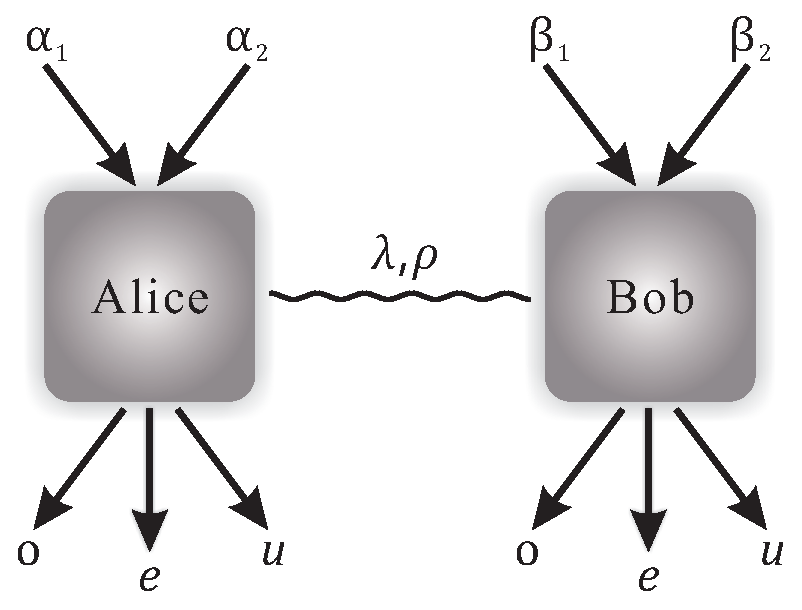
\includegraphics[scale=1]{epsCH.eps}}\\
  \caption{The CH inequality with two input settings and three possible outputs.}\label{Fig:CH}
\end{figure}

\paragraph{CH inequality:}
The CH inequality is a bipartite Bell inequality with measurement settings $x\in\{\alpha_1, \alpha_2\}$ and $y\in\{\beta_1, \beta_2\}$, and outputs $a,b\in\{o,e,u\}$, corresponding to ordinary, extraordinary, and undetected events, respectively. The CH inequality is defined by a linear combination of the probability distribution $p(a,b|x,y)$ by
\begin{equation}\label{eq:CHdef}
\begin{aligned}
  \bar{J} &= -p_{oo}(\alpha_1, \beta_1)  -p_{oo}(\alpha_1, \beta_2) -p_{oo}(\alpha_2, \beta_1)\\
  & +p_{oo}(\alpha_2, \beta_2)+ p_o^A(\alpha_1)  +p_o^B(\beta_1)  \geq 0.
   \end{aligned}
\end{equation}
Here, we take a more convenient notation of $p(a,b|x,y)$ as $p_{ab}(x,y)$, and $p_o^A(\alpha_1)$ ($p_o^B(\beta_1)$) refers to the probability of obtaining $o$ when Alice's (Bob's) input is $\alpha_1$ ($\beta_1$). It is easy to prove that the CH inequality is satisfied with all LVHMs.

In practice, we have to run many times to sample the probability distribution in Eq.~\eqref{eq:CHdef}. Suppose that the input setting is uniformly random and the number of each input setting is $N$, then the CH inequality can also be written as
\begin{equation}\label{eq:CH2}
\begin{aligned}
  N\bar{J} &\approx -n_{oo}(\alpha_1, \beta_1)  -n_{oo}(\alpha_1, \beta_2) -n_{oo}(\alpha_2, \beta_1) \\& +n_{oo}(\alpha_2, \beta_2)+ n_o^A(\alpha_1)/2  +n_o^B(\beta_1)/2  \geq 0.
   \end{aligned}
\end{equation}
Here, $n_{oo}(x, y)$ denotes coincidence detection of $oo$ with inputs $x$ and $y$, and  $n_o^A(x)$ ($n_o^B(y)$) denotes the single detection $o$ of Alice (Bob) with input $x$ ($y$). The factor of $2$ comes from the change from conditional probability to joint probability. Notice that, Eq.~\eqref{eq:CH2} is approximately satisfied for finite samples of $N$. It becomes the equal sign when $N$ goes to infinity.

\paragraph{Eberhard's inequality:}
In experiment, we can specify the single counts $n_o^A(\alpha_1)$ and $n_o^B(\beta_1)$ to be
\begin{equation}\label{eq:singlecounts}
\begin{aligned}
  n_o^A(\alpha_1)/2 &= n_{oo}(\alpha_1, \beta_2) + n_{oe}(\alpha_1, \beta_2) + n_{ou}(\alpha_1, \beta_2)\\
  n_o^B(\beta_1)/2 &= n_{eo}(\alpha_2, \beta_1)+n_{uo}(\alpha_2, \beta_1)+n_{oo}(\alpha_2, \beta_1)
   \end{aligned}
\end{equation}
Then, the CH inequality in finite runs can be expressed by
\begin{equation}\label{eq:Eberhard}
\begin{aligned}
  J_N &= -n_{oo}(\alpha_1, \beta_1) + n_{oe}(\alpha_1, \beta_2) + n_{ou}(\alpha_1, \beta_2)\\
  &+n_{eo}(\alpha_2, \beta_1)+n_{uo}(\alpha_2, \beta_1)+n_{oo}(\alpha_2, \beta_2) \geq 0,
\end{aligned}
\end{equation}
which is also known as the Eberhard's inequality. In the asymptotical limit, the relation between the CH inequality in Eq.~\eqref{eq:CHdef} and the Eberhard's inequality in Eq.~\eqref{eq:Eberhard} is
\begin{equation}\label{}
  \bar{J} = J_N/N.
\end{equation}

With the no-signaling assumption, we can prove that the CHSH, CH, and Eberhard's inequalities are equivalent.


\section{Quantum Teleportation}
The seminal work by C.~H.~Bennett, G.~Brassard, C.~Cr\'epeau, R.~Jozsa, A.~Peres and W.~K.~Wootters is published in 1993 \cite{PhysRevLett.70.1895}. Quantum teleportation is a process by which quantum information can be transmitted (exactly, in principle) from one location to another, with the help of classical communication and previously shared quantum entanglement between the sending and receiving location. Because it depends on classical communication, which can proceed no faster than the speed of light, it cannot be used for superluminal transport or communication of classical bits. It also cannot be used to make copies of a system, as this violates the no-cloning theorem.

\begin{figure}[hbt]
\centering \resizebox{6cm}{!}{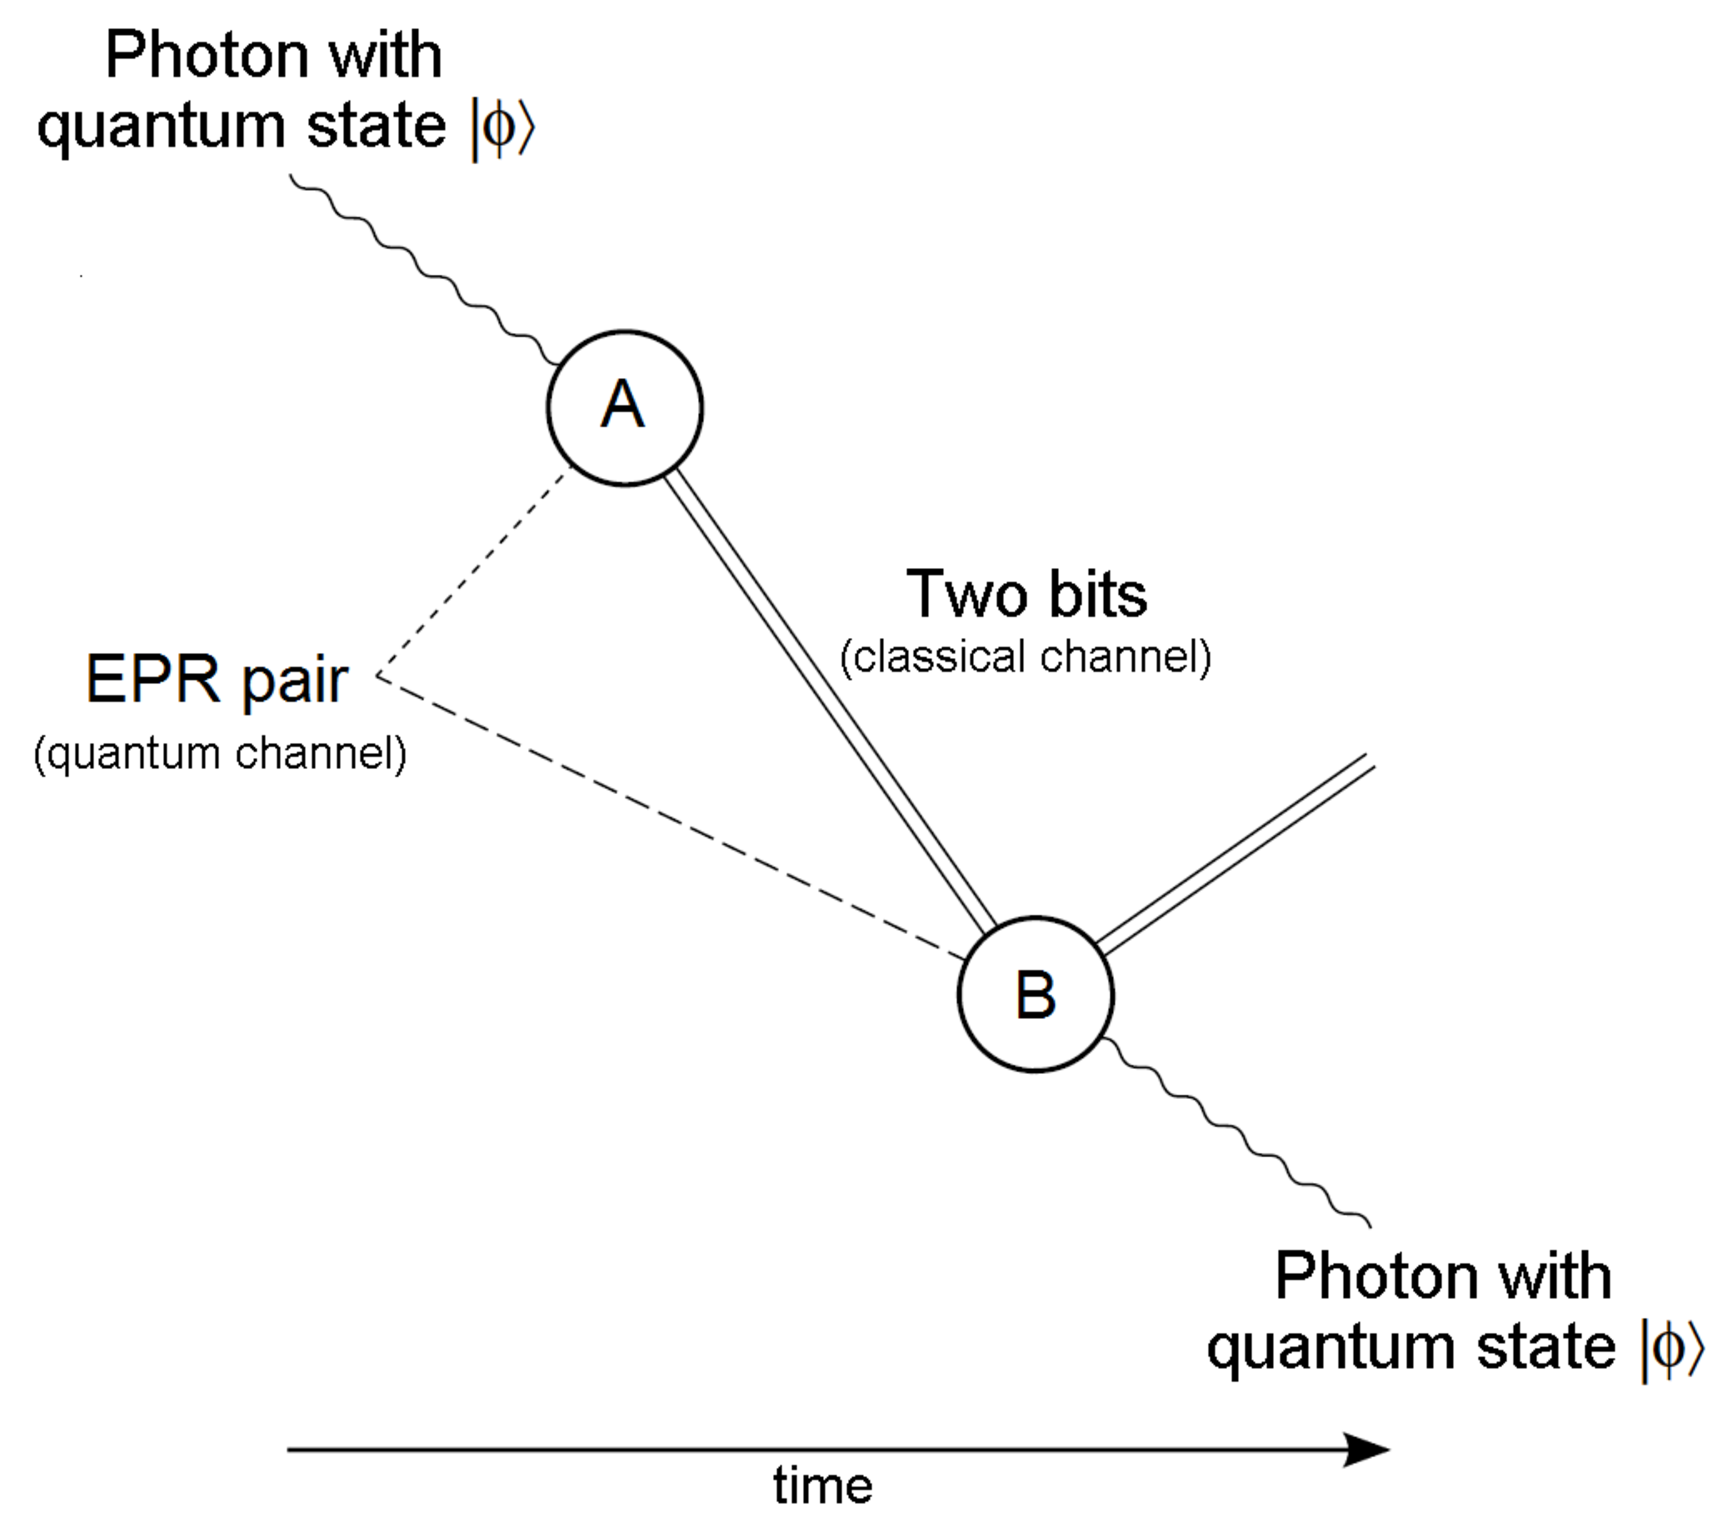
\includegraphics{epsTeleportation.eps}}
\caption{Schematic diagram for quantum teleportation.} \label{Fig:Teleport}
\end{figure}

Quantum teleportation can be regarded as a secure way to transfer information \cite{Lo1999Science}.

\subsection{A Quantum Teleportation protocol}

Alice can transfer Bob a qubit $a\ket{0} + b\ket{1}$by trivially sending $a$ and $b$ to Bob. Can we do better by sharing some entangled qubits?

Supposing that the qubit Alice wants to transfer to Bob is $a\ket{0}_E + b\ket{1}_E$, and also they share a EPR pair in common which is $\ket{0}_A\ket{0}_B + \ket{1}_A\ket{1}_B$.

We can check that
\begin{align}
&(a\ket{0}+b\ket{1})_E(\ket{00}+\ket{11})_{AB} \notag \\
=&(\ket{00}+\ket{11})_{EA}(a\ket{0}+b\ket{1})_B \notag \\
+&(\ket{01}+\ket{10})_{EA}(a\ket{1}+b\ket{0})_B \notag \\
+&(\ket{00}-\ket{11})_{EA}(a\ket{0}-b\ket{1})_B \notag \\
+&(\ket{01}-\ket{10})_{EA}(a\ket{1}-b\ket{0})_B \notag 
\end{align}

Thus, we can do teleportation using the following steps
\begin{itemize}
\item
Alice do a BSM(Bell-State measurement), and then sending her measurement result(2 bits) to Bob.
\item
Bob apply different unitary transformations based the bits Alice sent to him.
\end{itemize}

More specifically, Bob will apply
$$
\begin{cases}
I & \text{Alice got $\ket{00} + \ket{11}$} \\
\sigma_x & \text{Alice got $\ket{01} + \ket{10}$} \\
\sigma_z & \text{Alice got $\ket{00} - \ket{11}$} \\
\sigma_x\sigma_z & \text{Alice got $\ket{01} - \ket{10}$}
\end{cases}
$$

Thus we can see that
$$
2\text{bit} + 1\text{ebit} \ge 1\text{qubit}.
$$
\subsection{Teleportation of entanglement}

The teleportation also works for the entanglement state. The name of this work is entanglement swapping\cite{PhysRevLett.71.4287}.
\begin{figure}[hbt]
\centering \resizebox{6cm}{!}{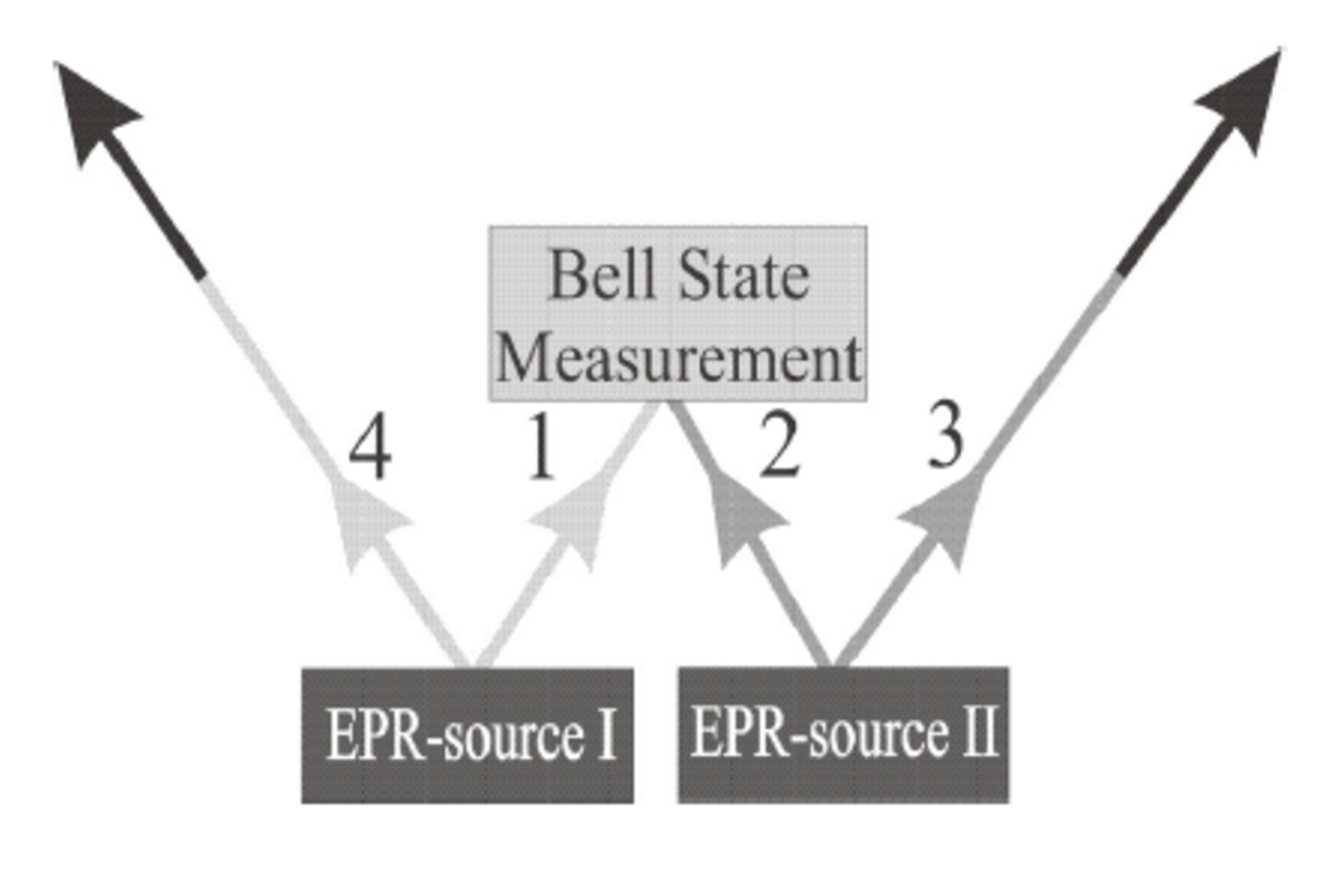
\includegraphics{epses.eps}}
\caption{Schematic diagram for entanglement swapping.} \label{Fig:entanglement swapping}
\end{figure}


\subsection{Experimental Realizations of quantum teleportation}
\begin{enumerate}[$*$]
\item D. Bouwmeester, et al., Nature 390, 575-579 (1997) (photons),
\item D. Boschi, et al., Phys. Rev. Lett. 80, 1121-1125 (1998) (photons),
\item J-W. Pan, et al., Phys. Rev. Lett. 80, 3891�C3894 (1998) (mixed state of
photons),
\item A. Frusawa, et al., Science 282, 706 (1999) (continuous-variable),
\item M. Riebe, et al., Nature 429, 734-737 (2004) (trapped calcium ions),
\item M.D. Barret, et al., Nature 429, 737-739 (2004) (trapped beryllium ions),
\item I. Marcikic, et al., Nature 421, 509-513 (2003) (long distance),
\item R. Ursin, et al., Nature 430, 849 (2004) (long distance),
\item Z. Zhao, et al., Nature 430, 54 (2004) (open destination teleportation).
\end{enumerate}


\section{Quantum Super dense coding}

At the beginning of the section, we will introduce the main idea of the Quantum Super dense coding.

As shown in Eq.~\eqref{4BellZ}, the four Bell states in the $Z$ basis are,
\begin{equation} \label{4BellZreview}
\begin{aligned}
\ket{\Phi^+} &= \ket{00}+\ket{11} \\
\ket{\Phi^-} &= \ket{00}-\ket{11} \\
\ket{\Psi^+} &= \ket{01}+\ket{10} \\
\ket{\Psi^-} &= \ket{01}-\ket{10} \\
\end{aligned}
\end{equation}

Each of the Bell states can transform to an arbitrary target Bell state through one of unitary operations ($\{\sigma_I,\sigma_X,\sigma_Y,\sigma_Z\}$) applied on the first qubit. For example, when the target Bell state is $\ket{\Phi^+}$,

\begin{equation} \label{4BellZnew}
\begin{aligned}
\ket{\Phi^+} &= \ket{00}+\ket{11}= \sigma_I\ket{\Phi^+}\\
\ket{\Phi^-} &= \ket{00}-\ket{11}=\sigma_Z\ket{\Phi^+} \\
\ket{\Psi^+} &= \ket{01}+\ket{10}=\sigma_X\ket{\Phi^+} \\
\ket{\Psi^-} &= \ket{01}-\ket{10}=-i\sigma_Y\ket{\Phi^+} \\
\end{aligned}
\end{equation}

\subsection{Quantum Super dense coding protocol}

Classical: 1 channel can only transfer 1 bit.

Aim: transfer 2 bits by transfer just 1 qubit.

Alice and Bob hold a Bell state, say $\ket{0}_A\ket{0}_B + \ket{1}_A\ket{1}_B$, in common.

Once Alice have two qubits of information, say $i_0i_1$, to send to Bob, she applies one of the following measurements based on $i_0i_1$: 
$$
\begin{cases}
I & i_0i_1 = 00 \\
\sigma_{xA} & i_0i_1 = 01 \\
\sigma_{zA} & i_0i_1 = 10 \\
\sigma_{xA}\sigma_{zA} & i_0i_1 = 11
\end{cases}
$$

We can verify that, after applying these operations,
$$
\begin{cases}
\ket{00}+\ket{11} \xrightarrow{I} \ket{00}+\ket{11} \\
\ket{00}+\ket{11} \xrightarrow{\sigma_{xA}} \ket{10}+\ket{01} \\
\ket{00}+\ket{11} \xrightarrow{\sigma_{zA}} \ket{00}-\ket{11} \\
\ket{00}+\ket{11} \xrightarrow{\sigma_{xA}\sigma_{zA}} \ket{01}-\ket{10}
\end{cases}
$$

Bob can then simply achieve the information Alice sent to him by a Bell-State measurement.

We can then illustrate that 
$$
1\text{qubit} + 1\text{ebit(entangled bit)} \ge 2\text{bit}.
$$

\section{Remote State Preparation}
Different from the teleportation, the initial state is known to Alice and unknown to Bob. In teleportation, to recover the initial state, Alice require to tell Bob the result of BSM which requires 2 bits of classical information. In the remote state preparation scenario, an equatorial state $\ket{\psi}=\ket{0}+e^{i\theta}\ket{1}$ can be transmitted to be with 1 bit of classical information.

Alice owns a qubit $\ket{\phi}$, and she wants Bob to get $\ket{\phi}$. Assuming that they share a EPR pair, say $\ket{00} + \ket{11}$ in common. 
\subsection{Send $\ket{0}$}

Alice apply a $\sigma_z$ measurement on the qubit she owned in the EPR pair. If she got $\ket{0}$, then she tells Bob do nothing. Otherwise, she knows that the qubit that Bob owns will definitely be $\ket{1}$, thus she tells Bob to apply a $\sigma_x$ transformation to flip the qubit.
\subsection{Send $\ket{+}$}

Alice apply a $\sigma_x$ measurement on the qubit she owned in the EPR pair. If she got $\ket{+}$, then she tells Bob do nothing. Otherwise, she knows that the qubit that Bob owns will definitely be $\ket{-}$, thus she tells Bob to apply a $\sigma_x$ transformation to flip the qubit.

\subsection{General Case with real}

Supposing $\ket{\phi} = a\ket{0} + b\ket{1}$, and assuming that $a, b \in \mathbb{R}$.

We know that for real $\ket{\phi} = a\ket{0} + b\ket{1}$ where $a$ and $b$ are real, we have
$$
\ket{00} + \ket{11} = \ket{\phi\phi} + \ket{\phi^{\perp}\phi^{\perp}}.
$$

Alice can first do a measurement based on $\ket{\phi}$ and $\ket{\phi^{\perp}}$, and if she gets $\ket{\phi}$, then she told Bob to do nothing. Otherwise, she told Bob to transform from $\ket{\phi^{\perp}}$ to $\ket{\phi}$.

However, such transformations, i.e., to transform from $\ket{\phi^{\perp}}$ to $\ket{\phi}$, is only independent of $\ket{\phi}$ when $a, b \in \mathbb{R}$. Actually we don't have such universal gate in the scenario that $a, b \in \mathbb{C}$.

\subsection{A Special Case with image}
First, Alice and Bob share a bell state $\ket{\Psi^-} = \ket{01}-\ket{10}$. Then Alice measures her state in the $\{ \ket{\psi},\ket{\psi^\perp}\}$ basis, where $\ket{\psi^\perp}=\ket{0}-e^{i\theta}\ket{1}$.
The bell state can be write as $\ket{\psi}\ket{\psi^\perp}-\ket{\psi^\perp}\ket{\psi}$. When Alice's result is $\ket{\psi^\perp}$, Bob' state is the initial state $\ket{\psi}$. When Alice's result is $\ket{\psi}$, Bob's state is $\ket{\psi^\perp}$ which requires to apply a $Z$ operation. For a general state, the number of classical can also be 1, but requires 3.79 bits of the ebits.

\section{Using teleportation for operation (Gottesman-Chuang'99)}

We know that universal quantum computation can be achieved with CNOT gates and single qubit operations. In this section, we will show how to construct a CNOT gate using teleportation (Fig.~
\ref{Fig:CNOT}). The result of the BSM $B$ is

\begin{equation} \label{BSM}
\begin{aligned}
\ket{\Phi^+} &= \ket{00}+\ket{11}:00\\
\ket{\Phi^-} &= \ket{00}-\ket{11}:01 \\
\ket{\Psi^+} &= \ket{01}+\ket{10}:10 \\
\ket{\Psi^-} &= \ket{01}-\ket{10}:11 \\
\end{aligned}
\end{equation}
The teleportation is shown as following,

\begin{figure}[hbt]
\centering \resizebox{6cm}{!}{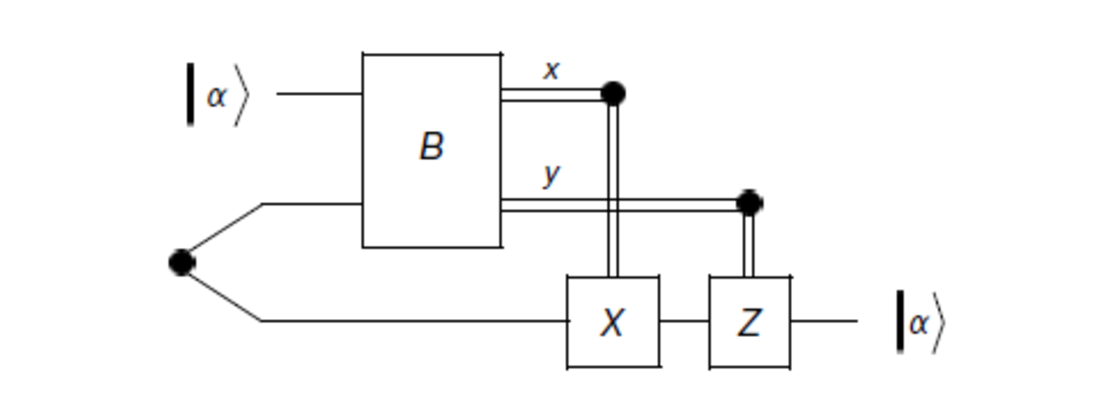
\includegraphics{epsTeleportation1.eps}}
\caption{Schematic diagram for teleportation.} \label{Fig:teleportation1}
\end{figure}


\begin{figure}[hbt]
\centering \resizebox{6cm}{!}{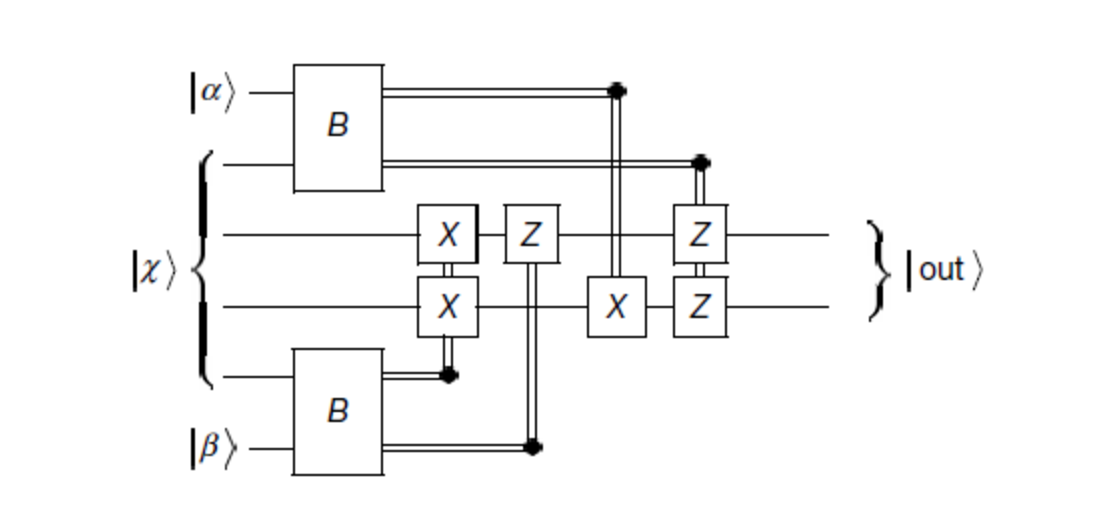
\includegraphics{epsCNOT.eps}}
\caption{Schematic diagram for CNOT gate using teleportation, where $\ket{\chi}=(\ket{00}+\ket{11})\ket{00}+(\ket{01}+\ket{10})\ket{11}$.} \label{Fig:CNOT}
\end{figure}

The state $\ket{\chi}=(\ket{00}+\ket{11})\ket{00}+(\ket{01}+\ket{10})\ket{11}$ can be prepared as following,
\begin{figure}[hbt]
\centering \resizebox{6cm}{!}{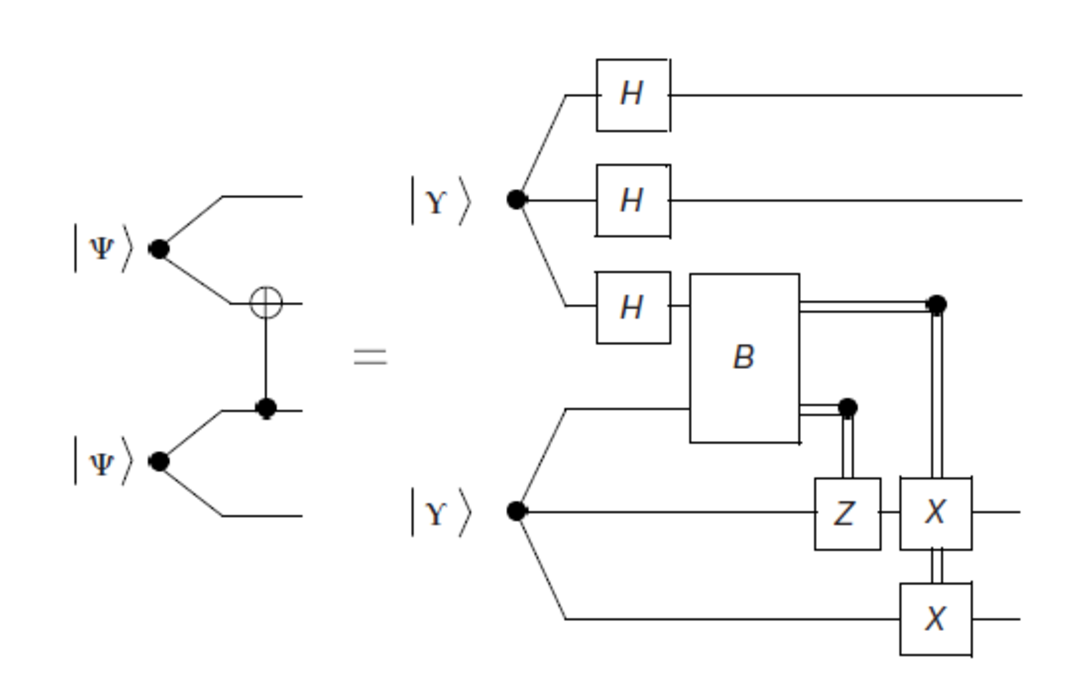
\includegraphics{epschi.eps}}
\caption{Schematic diagram for $\ket{\chi}$, where $\ket{\gamma}=\ket{000}+\ket{111}$.} \label{Fig:CHI}
\end{figure}



%%%%%%%%%%%%%%%%%%%%%%%%%%%%%%%%%%%%%%%%
% choose a style
%\bibliographystyle{ieeetr}
%\bibliographystyle{unsrt}
\bibliographystyle{apsrev4-1}
%%%%%%%%%%%%%%%%%%%%%%%%%%%%%%%%%%%%%%%%


%%%%%%%%%%%%%%%%%%%%%%%%%%%%%%%%%%%%%%%%
% choose a .bib file
\bibliography{bibAdvQI}
%%%%%%%%%%%%%%%%%%%%%%%%%%%%%%%%%%%%%%%%
\end{document}
